\section{Тюнинг SVM классификатора}
Изучим влияние значения {\it параметра штрафной функции SVM классификатора} на
качество оценки.
Этот параметр определяет величину отступа для разделения классов при построении
модели, и обозначается $Cost$.

Оценки, полученные в п. \ref{sec:sentirueval2015} и \ref{sec:sentirueval2016},
были получены при значении такого параметра по-умолчанию, т.е. $Cost=1$.
Посмотрим, как будет изменяться результат, если уменьшить величину отступа для
разделения классов.
Для тестирования используются такие обучающие коллекции, на которых ранее были
получены наилучшие результаты (см. таблицы \ref{table:results2015}, \ref{table:results2016})
на рис. \ref{fig:cost} представлено изменение качества работы моделей в
зависимости от изменения параметра $Cost$.

\begin{figure}[!htp] \centering
    \captionsetup[subfigure]{justification=centering}
    \begin{subfigure}[b]{0.45\textwidth}
        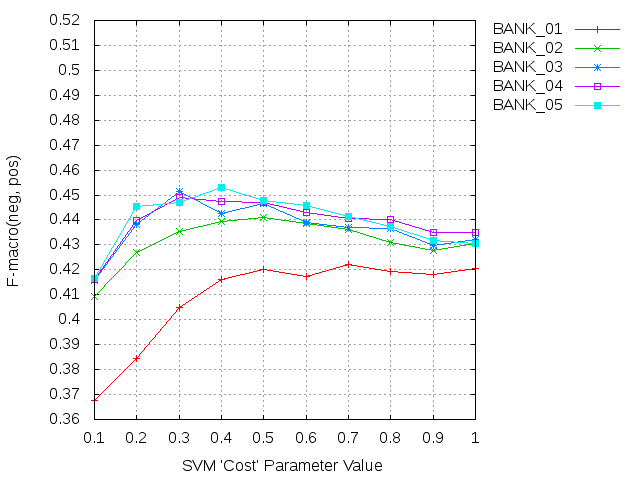
\includegraphics[width=\textwidth]{pics/2015_bank_balanced.png}
        \caption{$B_{bank}^{15}$, BANK'15}
        \label{fig:bank_cost_changes_2015}
    \end{subfigure}
    ~
    \begin{subfigure}[b]{0.45\textwidth}
        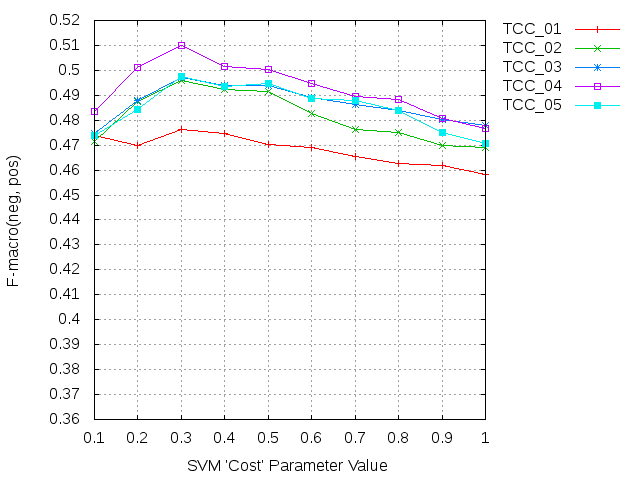
\includegraphics[width=\textwidth]{pics/2015_ttk_balanced.png}
        \caption{$I_{tcc}^{15}$, TCC'15}
        \label{fig:tcc_cost_changes_2015}
    \end{subfigure}

    \begin{subfigure}[b]{0.45\textwidth}
        \includegraphics[width=\textwidth]{pics/2016_bank_imbalanced.png}
        \caption{$I_{bank}^{16}$, BANK'16}
        \label{fig:bank_cost_changes_2016}
    \end{subfigure}
    ~
    \begin{subfigure}[b]{0.45\textwidth}
        \includegraphics[width=\textwidth]{pics/2016_ttk_balanced.png}
        \caption{$B_{tcc}^{16}$, TCC'16}
        \label{fig:tcc_cost_changes_2016}
    \end{subfigure}

    \caption{
        Влияние {\it параметра штрафной функции SVM классификатора}
        на результаты прогонов;
        кривыми на графиках обозначается прогоны с соответсвующими номерами;
        значение параметра измерялось в пределе $[0.1, 1]$ с шагом $0.1$.
    }
    \label{fig:cost}
\end{figure}

Сравнивая резулататы для данных '15 и '16 года по каждой из задачи, можно
наблюдать примерно схожую картину поведения моделей. Например, для задачи
BANK (рис. \ref{fig:bank_cost_changes_2015}, \ref{fig:bank_cost_changes_2016})
засчет большего объема обучающих данных в $I_{bank}^{16}$ при тестировании на
$SentiRuEval-2016$ заметен прирост существенный прирост качества работы модели,
при $Cost \in \left[0.5, 1\right]$.
Дальнейшее уменьшение этого параметра существенно снижает качество
оценки, что говорит о расхождении данных обучающей и тестовых коллекций.

Если рассмотреть результаты отностельно задачи TCC (рис.
\ref{fig:tcc_cost_changes_2015}, \ref{fig:tcc_cost_changes_2016}),
прирост качества наблюдается в диапазоне $Cost \in [0.3, 0.5]$.
Провал в результатах при использования меньших значений параметра
не так сильно выражен, что объясняет лучшую разделимость классов.

Если сравнивать результаты обучения на сбалансированных (рис.
\ref{fig:bank_cost_changes_2015}, \ref{fig:tcc_cost_changes_2016}) и не
сбалансированных (\ref{fig:tcc_cost_changes_2015}, \ref{fig:bank_cost_changes_2016})
коллекциях, то во втором случае, при изменении Cost параметра, колебания
результата выражены сильнее. Правильно подобранные сообщения для балансировки
может позволить добиться лучшего результата при уменьшении параметра $Cost$.

